\section{Protolys}

Protolys\footnote{se s. 60 i boken}---från \emph{proto} för proton och forngrekiskans \emph{lúsis} för lossa---innebär att det sker ett utbyte av en eller flera protoner ($\ce{H+}$ joner). Som angivet ovan kommer syror lossa en proton och baser ta emot en.
\begin{exm}
    Låt en syra A som innehåller en väteatemom H reagera med vatten. Detta kallas också att den \emph{protolyseras}:
    \begin{center}
        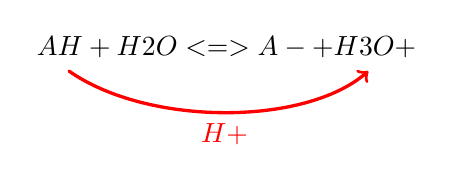
\begin{tikzpicture}
            \node at (0,0) {$\ce{AH + H2O <=> A- + H3O+}$};
            \draw[very thick, color=red, ->, line cap=round] (-2,-0.3) .. controls (-1,-1) and (1,-1) .. node[anchor=north] {$\ce{H+}$} (1.8,-0.3);
        \end{tikzpicture}
    \end{center}
    Något mycket liknande sker när en bas B protolyseras:
    \begin{center}
        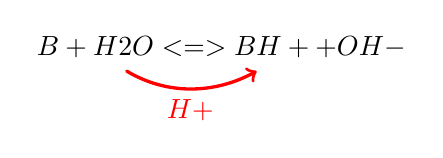
\begin{tikzpicture}
            \node at (0,0) {$\ce{B + H2O <=> BH+ + OH-}$};
            \draw[very thick, color=red, ->, line cap=round] (-1.2,-0.3) .. controls (-0.7,-0.6) and (-0.1,-0.6) .. node[anchor=north] {$\ce{H+}$} (0.45,-0.3);
        \end{tikzpicture}
    \end{center}
\end{exm}

\section{pH och pOH}

Dessa är ett mått på hur syrligt eller basiskt en lösning är. pH är absolut standard med det finns anvädningar för pOH också. Skalan är logaritmisk med bas 10 och går från ca -1 till ca 14. Definitionen för de två storheterna är:
\begin{align*}
    \mathrm{pH} &= -\log{\ce{[H3O+]}} \\
    \mathrm{pOH} &= -\log{\ce{[OH^-]}}
\end{align*}
Ju högre pH är desto mer basiskt och ju mer basiskt desto mindre desto mer syrligt. En neutral lösning har pH 7. Då är $\ce{[H3O+] = [OH^-]}$. För att beräkna ena eller andra vet vi även detta samband:
\[
    \mathrm{pH + pOH} = 14
\]